\pdfminorversion=4
\documentclass[]{beamer}
\mode<presentation>

% beamer stuff
% Gives us the bottom line with all the goodies
\useoutertheme{infolines}
% Just the theme to use. Should be built into bemaer. Setting the
% height gets rid of a whole lot of whitespace
\usetheme[height=7mm]{Rochester}
\usefonttheme{serif}
% Usually beamer gives you navigation hyperlinks on the bottom
% right. I turned this off. It's annoying.
\setbeamertemplate{navigation symbols}{} 
% Makes my text boxes look pretty
\setbeamertemplate{blocks}[rounded][shadow=true] 
% Makes my bullet points 3d balls
\setbeamertemplate{items}[ball]

% Josh's packages
\usepackage{multimedia}
\usepackage{graphicx}

% Packages for me
\usepackage{amsmath,amssymb,latexsym,amsthm}
\usepackage[mathscr]{eucal}
\usepackage{mathrsfs}
\usepackage{verbatim}
\usepackage{braket}
\usepackage{listings}
\usepackage{xcolor}
% \usepackage[usenames,dvipsnames,svgnames,table]{xcolor}
\usepackage{fancybox}
\usepackage{animate}
% \usepackage{media9}
\usepackage{multicol}
\usepackage{mdframed}
\usepackage{hyperref}
%\usepackage{scalerel}
\usepackage[outline]{contour}
\contourlength{1.2pt}

% Macros

%Blackboard Bold
\newcommand{\R}{\mathbb{R}}
\newcommand{\Z}{\mathbb{Z}}
\newcommand{\N}{\mathbb{N}}
\newcommand{\Q}{\mathbb{Q}}
\newcommand{\A}{\mathbb{A}}
\newcommand{\E}{\mathbb{E}}
% other
\newcommand{\eval}{\biggr\rvert} %evaluated at
\newcommand{\myvec}[1]{\mathbf{#1}} % vectors for me
% total derivatives 
\newcommand{\diff}[2]{\frac{d #1}{d #2}} 
\newcommand{\dd}[1]{\frac{d}{d #1}}
% partial derivatives
\newcommand{\pd}[2]{\frac{\partial #1}{\partial #2}} 
\newcommand{\pdd}[1]{\frac{\partial}{\partial #1}} 
% Order operator
\DeclareRobustCommand{\orderof}{\ensuremath{\mathcal{O}}}

% braces
\newcommand{\paren}[1]{\left( #1 \right)}
\newcommand{\sqrbrace}[1]{\left[ #1 \right]}
\newcommand{\curlybrace}[1]{\left\{ #1 \right\}}
\newcommand{\inner}[1]{\paren{#1}}
\newcommand{\norm}[1]{\left| #1 \right|_2}

% g
\newcommand{\detg}{\sqrt{-g}}

% neutrinos
\newcommand{\eepsilon}{\epsilon} % energy
\newcommand{\fin}{f\in \{\nu_e,\nu_{\bar{e}},\nu_x\}}
\newcommand{\sign}{\text{sign}(f)}
\newcommand{\jnuf}{j_{\eepsilon,f}}
\newcommand{\etanuf}{\eta_{\eepsilon,f}}
\newcommand{\Inuf}{I_{\eepsilon,f}}
\newcommand{\chinuf}{\chi_{\eepsilon,f}}
\newcommand{\sigmanuf}{\sigma_{\eepsilon,f}}
\newcommand{\alphanuf}{\alpha_{\eepsilon,f}}
\newcommand{\numin}{\nu_{\text{min}}}
\newcommand{\numax}{\nu_{\text{max}}}


% tikz
% tikz
\usepackage{tikz}
\usepackage{pgfplots}
\usetikzlibrary{calc,fadings,decorations.pathreplacing}
\usetikzlibrary{arrows}
\usetikzlibrary{decorations.pathmorphing}
\usetikzlibrary{decorations.markings}
\usetikzlibrary{arrows.meta,bending}

% Keys to support piece-wise uncovering of elements in TikZ pictures:
% \node[visible on=<2->](foo){Foo}
% \node[visible on=<{2,4}>](bar){Bar}   % put braces around comma expressions
% 
% Internally works by setting opacity=0 when invisible, which has the 
% adavantage (compared to \node<2->(foo){Foo} that the node is always there, hence
% always consumes space plus that coordinate (foo) is always available.
% 
% The actual command that implements the invisibility can be overriden
% by altering the style invisible. For instance \tikzsset{invisible/.style={opacity=0.2}}
% would dim the "invisible" parts. Alternatively, the color might be set to white, if the
% output driver does not support transparencies (e.g., PS) 
% 
\tikzset{
  invisible/.style={opacity=0},
  visible on/.style={alt={#1{}{invisible}}},
  alt/.code args={<#1>#2#3}{%
    \alt<#1>{\pgfkeysalso{#2}}{\pgfkeysalso{#3}} % \pgfkeysalso doesn't change the path
  },
}

% some nice flowchart features
\tikzset{
    mynode/.style={rectangle,rounded corners,draw=black, top color=white, bottom color=yellow!50,very thick, inner sep=1em, minimum size=3em, text centered},
    myimgnode/.style={rectangle,rounded corners,draw=black, top color=white, bottom color=yellow!50,very thick, inner sep=0.25em, minimum size=3em, text centered},
    myarrow/.style={->, >=latex', shorten >=2pt, thick},
    mylabel/.style={text width=8em, text centered} 
}  

% squigly arrow
\tikzset{zigzag it/.style={decorate, decoration=zigzag}}

% Color morphing arrow
\tikzset{colormorph/.style n args={3}{
    postaction={
    decorate,
    decoration={
    markings,
    mark=between positions 0 and \pgfdecoratedpathlength step 0.5pt with {
    \pgfmathsetmacro\myval{multiply(
        divide(
        \pgfkeysvalueof{/pgf/decoration/mark info/distance from start}, \pgfdecoratedpathlength
        ),
        100
    )};
    \pgfsetfillcolor{#3!\myval!#2};
    \pgfpathcircle{\pgfpointorigin}{#1};
    \pgfusepath{fill};}
}}}}

% define a really nice visible "purple"
\definecolor{gimppurple}{HTML}{AD26FB}
% a light grey
\definecolor{lightgrey}{HTML}{E0E0E0}
% for highlighting
\definecolor{deepblue}{rgb}{0,0,0.5}
\definecolor{deepred}{rgb}{0.6,0,0}
\definecolor{deepgreen}{rgb}{0,0.5,0}

% fonts
% Default fixed font does not support bold face
\DeclareFixedFont{\ttb}{T1}{txtt}{bx}{n}{12} % for bold
\DeclareFixedFont{\ttm}{T1}{txtt}{m}{n}{12}  % for normal

% Python style for highlighting
\newcommand\pythonstyle{\lstset{
language=Python,
basicstyle=\ttm,
otherkeywords={self},
keywordstyle=\ttb\color{deepblue},
emph={__init__},           
emphstyle=\ttb\color{deepred},
commentstyle=\ttfamily\color{deepred},
stringstyle=\color{deepgreen},
frame=tb,                     
showstringspaces=false        
}}

% Python environment
\lstnewenvironment{python}[1][]
{
\pythonstyle
\lstset{#1}
}
{}

\newcommand{\backupbegin}{
   \newcounter{finalframe}
   \setcounter{finalframe}{\value{framenumber}}
}
\newcommand{\backupend}{
   \setcounter{framenumber}{\value{finalframe}}
}

% Automatically generates section breaker slides
\AtBeginSection[]{
  \begin{frame}[plain]
  \vfill
  \centering
  \begin{beamercolorbox}[sep=8pt,center,shadow=true,rounded=true]{title}
    \usebeamerfont{title}\insertsectionhead\par%
  \end{beamercolorbox}
  \vfill
  \end{frame}
}

\title[Nuclear Astro]{Nuclear Astrophysics and Astrophysical Transients}
% \subtitle{Models and Implications}
\author[J. Miller]{Jonah Miller}
% \author[J. Miller]{\textcolor{blue}{Jonah M. Miller},\\
%   S. Curtis, V. Urrutia-Hurtado, K. Lund, B. Barker\\
%   Many More...}
\institute[LANL]{Los Alamos National Laboratory}
% \titlegraphic{\vspace{1cm}}
% \titlegraphic{\includegraphics[height=0.25\textheight]{3d_render}}
\date[Dec 2022]{Hamburg}

\graphicspath{{figures/}}

\begin{document}

\begin{frame}[plain]
    \tikz [remember picture, overlay] 
    \node at ([xshift=2cm,yshift=-2cm]current page.west)
    {\includegraphics[width=0.25\textwidth,clip,trim={150 0 150 0}]{3d_render}};
    \tikz [remember picture, overlay] 
    \node at ([xshift=-2cm,yshift=-2cm]current page.east)
    {\includegraphics[width=0.25\textwidth,clip,trim={0 0 0 0}]{visit0006-gimp3}};
  \titlepage
\end{frame}

\begin{frame}[plain]
  \begin{itemize}
  \item This Document cleared for unlimited release with LA-UR-XX-XXXX
  \item The submitted materials have been authored by an employee or
    employees of Triad National Security, LLC (Triad) under contract
    with the U.S.  Department of Energy/National Nuclear Security
    Administration (DOE/NNSA).  Accordingly, the U.S. Government
    retains an irrevocable, nonexclusive, royalty- free license to
    publish, translate, reproduce, use, or dispose of the published
    form of the work and to authorize others to do the same for
    U.S. Government purposes.”
  \end{itemize}
\end{frame}

\begin{frame}
  \frametitle{SN1987A}
  \begin{columns}
    \begin{column}{5cm}
      \begin{itemize}
      \item Feb. 23, 1987
      \end{itemize}
      \begin{center}
        \includegraphics[height=0.6\textheight]{sn1987a-eso}\\
        ESO/Schmidt
      \end{center}
    \end{column}
    \begin{column}{7cm}
      \begin{itemize}
      \item Sept. 2, 2010
      \end{itemize}
      \begin{center}
        \includegraphics[height=0.6\textheight]{sn1987a-remnant}\\
        NASA/Hubble
      \end{center}
    \end{column}
  \end{columns}
\end{frame}

\begin{frame}
  \frametitle{Stellar structure primer}
  \begin{center}
    \includegraphics[height=0.75\textheight]{Nucleosynthesis_in_a_star}
  \end{center}
  Wikimedia Commons
\end{frame}

\begin{frame}
  \frametitle{Collapse}
  \begin{center}
    \includegraphics[height=0.7\textheight]{Core_collapse_scenario}
  \end{center}
  Hall, Magasjukur2, Wikimedia Commons
\end{frame}

\begin{frame}
  \frametitle{Powering The Explosion}
  \begin{center}
    \includegraphics[height=0.7\textheight]{neutrino-mechanism-janka}
  \end{center}
  T. Janka
\end{frame}

\begin{frame}
  \frametitle{Neutron Stars}
  \begin{center}
    \includegraphics[width=0.9\textwidth]{ns-manhattan}
  \end{center}
  Wikimedia Commons
\end{frame}

\begin{frame}
  \frametitle{The Nuclear Equation of State}
  \begin{columns}
    \begin{column}{6cm}
      \begin{center}
        \includegraphics[width=\columnwidth]{LonardoniTewesGandolfiCarlsonFig2}
      \end{center}
      Lonardoni et al., PRR \textbf{2} 022033 (2020)
    \end{column}
    \begin{column}{6cm}
      \begin{center}
        \includegraphics[width=\columnwidth]{ccsn-stats/ns-mass-rad}
      \end{center}
      Image from Carla Frohlich
    \end{column}
  \end{columns}
\end{frame}

\begin{frame}
  \frametitle{Nuclear EOS Impacts Explosion and Remnant}
  \begin{center}
    \includegraphics[height=0.7\textheight]{neutrino-mechanism-janka}
  \end{center}
  T. Janka
\end{frame}

\begin{frame}
  \frametitle{Observation vs Theory}
  \resizebox{12cm}{!}{
    \begin{tikzpicture}[node distance=9em]
      \node[myimgnode](star)
      {\includegraphics[width=6em]{Nucleosynthesis_in_a_star}};
      \node[myimgnode, right of=star](exp)
      {\includegraphics[width=6em]{neutrino-mechanism-janka}};
      \node[myimgnode, right of=exp](remnant)
      {\includegraphics[width=6em,clip,trim={500 0 0 0}]{ns-manhattan}};

      \node[mylabel, below of=exp] (sim) {simulation};

      \draw[myarrow] (star) -- (exp);
      \draw[myarrow] (exp) -- (remnant);

      \draw[myarrow] (sim) -- (exp);

      \draw[red] (-1,-2) -- ++(0.6, -0.25)
      -- ++(0.6, -0.5)
      -- ++(0.8, -1.25);

      \draw[ultra thick, black, ->] (-1, -4) -- ++(2.25, 0)
      node[below]{$M_{ZAMS}$};
      \draw[ultra thick, black, ->] (-1, -4) -- ++(0, 2.25)
      node[left]{pdf};

      \draw[domain=6:8, smooth, variable=\x, color=blue]
      plot ({\x}, {1.75*exp(-(\x-7)*(\x-7)/(0.25)) - 4});

      \draw[ultra thick, black, ->] (6, -4) -- ++(2.25, 0)
      node[below]{$M_{NS}$};
      \draw[ultra thick, black, ->] (6, -4) -- ++(0, 2.25)
      node[left]{pdf};
      
    \end{tikzpicture}
  }
\end{frame}

\begin{frame}
  \frametitle{Compare Distributions!}
  \begin{center}
    \includegraphics[height=0.9\textheight]{ccsn-stats/ns_kde_0p1}
  \end{center}
  Meskhi,...,\textbf{JMM} et al., ApJL \textbf{932} L3 (2022)
\end{frame}

\begin{frame}
  \frametitle{...Implies constraints on EOS!}
  \begin{center}
    \includegraphics[height=0.9\textheight]{ccsn-stats/delta-distances}
  \end{center}
  Meskhi,...,\textbf{JMM} et al., ApJL \textbf{932} L3 (2022)
\end{frame}

\begin{frame}
  \frametitle{Cosmic Gold}
  \begin{center}
    \includegraphics[width=0.9\textwidth]{quantagold_19201}
  \end{center}
  Ashley Mackenzie for Quanta Magazine, March 23, 2017
\end{frame}

\begin{frame}
  \frametitle{The 170817 Merger}
  \begin{center}
    \includegraphics[height=7cm]{abbot-timeline}
  \end{center}
  Abbot+, 2017
\end{frame}

\begin{frame}
  \frametitle{Neutron Star Mergers: A 2+ Component Model}
  \begin{columns}
    \begin{column}{6cm}
      \begin{center}
        \includegraphics[width=0.9\textwidth]{frames/betabin_000}
        % \animategraphics[width=0.9\textwidth,every=10,autoplay,loop,controls]
        % {5}{frames/betabin_}{000}{374}
      \end{center}
    \end{column}
    \begin{column}{6cm}
      \begin{center}
        \resizebox{\columnwidth}{!}{
          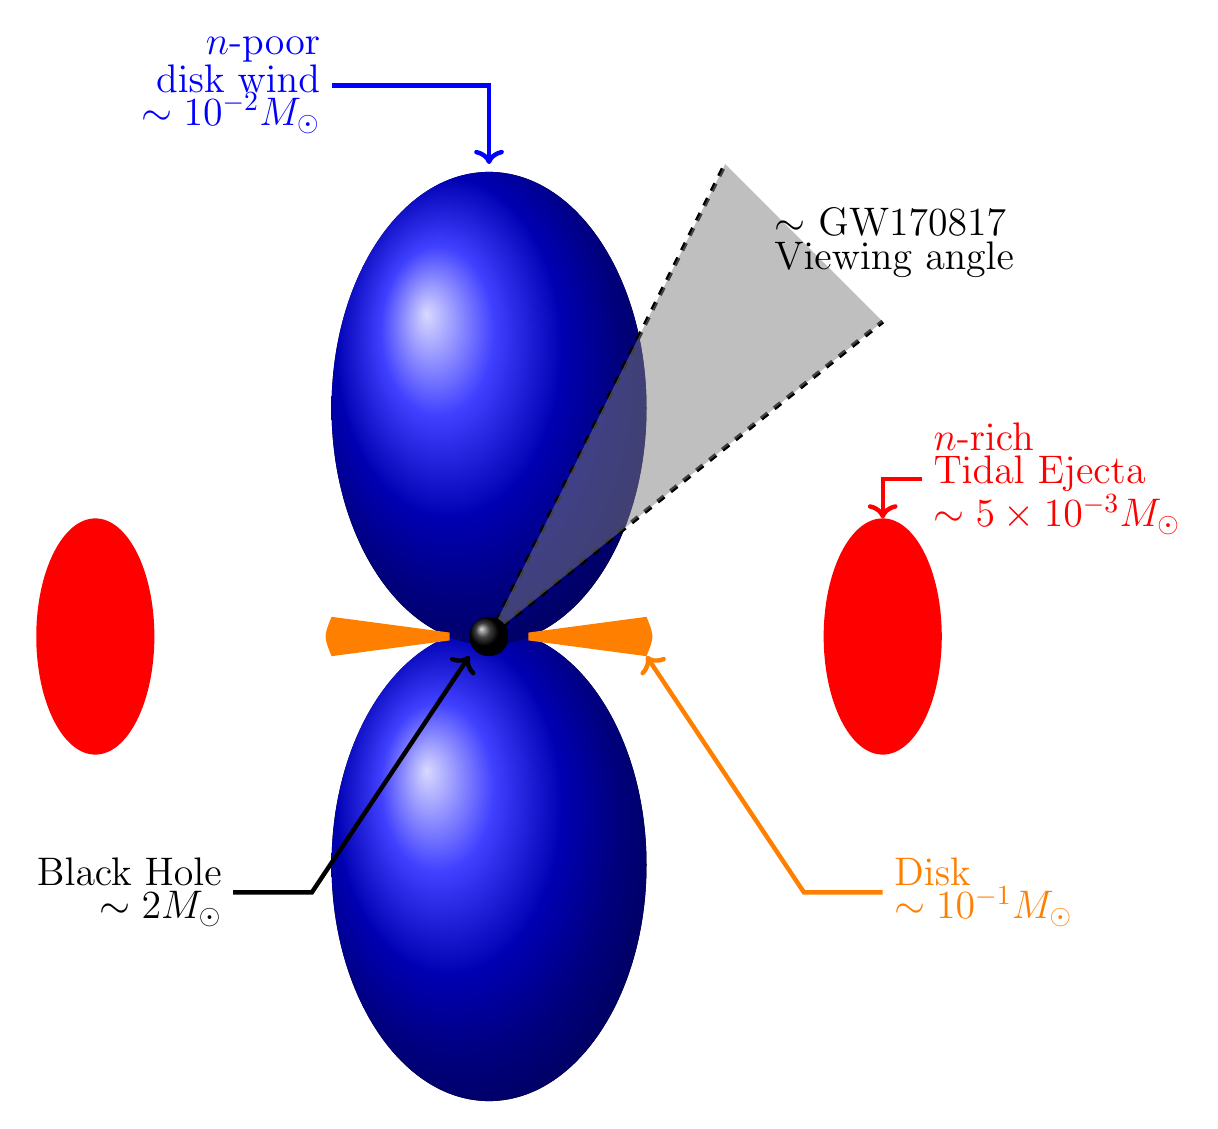
\begin{tikzpicture}
            \coordinate (origin) at (0,0);
            \pgfmathsetmacro{\dbx}{0.5}
            \pgfmathsetmacro{\dby}{0.05}
            \pgfmathsetmacro{\dex}{2.}
            \pgfmathsetmacro{\dey}{0.25}
            \pgfmathsetmacro{\dcc}{2.1}
            \pgfmathsetmacro{\tcx}{5.0}

            \foreach \i in {-1,1}
            {
              \fill[ball color=blue] (0, \i*2.9) ellipse (2 and 3);
            }

            \foreach \i in {-1,1}
            {
              % disk
              \fill[color=orange]
              (\i*\dbx,\dby) -- (\i*\dex,\dey)
              .. controls (\i*\dcc,0) .. (\i*\dex,-\dey)
              -- (\i*\dbx,-\dby) -- cycle;

              % tidal ejecta
              \fill[color=red] (\i*\tcx,0) ellipse (0.75 and 1.5);
            }

            % viewing
            \draw[dashed,ultra thick,black] (origin) -- (5,4);
            \draw[dashed,ultra thick,black] (origin) -- (3,6);
            \fill[color=gray,opacity=0.5] (origin) -- (5,4) -- (3,6) -- cycle;
            \node[right,align=left] at (3.5,5)
            {\Large $\sim$ GW170817\\ \Large Viewing angle};

            % bh
            \shade[ball color=black] (origin) circle (0.25);

            % text
            \draw[<-,red, ultra thick] (\tcx,1.5)
            -- ++(0.,0.5) -- ++(0.5,0)
            node[right,align=left]
            {\Large \color{red}$n$-rich\\\Large Tidal Ejecta\\ \Large $\sim 5\times 10^{-3}M_{\odot}$};

            \draw[<-,blue, ultra thick] (0,6) -- ++(0,1) -- ++(-2,0)
            node[left,align=right]
            {\Large \color{blue}$n$-poor\\\Large disk wind\\\Large $\sim 10^{-2}M_{\odot}$};

            \draw[<-,orange, ultra thick] (\dex,-\dey)
            -- ++(2,-3) -- ++(1,0)
            node[right,align=left]
            {\Large \color{orange}Disk\\\Large $\sim 10^{-1}M_{\odot}$};

            \draw[<-,black, ultra thick] (-0.25,-0.25)
            -- ++(-2,-3) -- ++(-1,0)
            node[left,align=right]
            {\Large \color{black}Black Hole\\ \Large $\sim 2 M_{\odot}$};
          \end{tikzpicture}
        }
      \end{center}
    \end{column}
  \end{columns}
  \begin{tiny}
    Co-design summer school, 2016
  \end{tiny}
\end{frame}

\begin{frame}
  \frametitle{The r-process}
  \begin{center}
   \includegraphics[width=0.9\textwidth]{skynet_ye_0p13/frame_0001}
  \end{center}
  Courtesy of J. Lippuner
\end{frame}

\begin{frame}
  \frametitle{The r-process}
  \begin{center}
    \includegraphics[width=0.9\textwidth]{skynet_ye_0p13/frame_0001}
    % \animategraphics[width=0.9\textwidth,every=5,autoplay,loop,controls]
    % {5}{skynet_ye_0p13/frame_}{0001}{0108}
  \end{center}
  Courtesy of J. Lippuner
\end{frame}

\begin{frame}
  \frametitle{Opacity}
  %\setlength{\unitlength}{1cm}
  \resizebox{12cm}{!}{
    \begin{tikzpicture}
      \node[inner sep=0pt] (rp) at (0,0)
      {\includegraphics[width=10cm]{skynet_ye_0p13/frame_0108}};
      \draw[ultra thick,red,<-] (1.5,-2) -- (2,-2.85)
      -- (2.25, -2.85) node[right] {\tiny Opaque to visible light};
      \draw[ultra thick,red,<-] (0.85,-2) -- (0.5,-2.85)
      -- (0.25,-2.85) node[left] {\tiny Not opaque};
    \end{tikzpicture}
  }
\end{frame}

\begin{frame}
  \frametitle{The Kilonova}
  \begin{center}
    \includegraphics[width=10cm]{swope-image}
  \end{center}
  M2H/UC Santa Cruz and Carnegie Observatories/Ryan Foley
\end{frame}

\begin{frame}
  \frametitle{Neutrino Transport Matters!}
  \begin{center}
    \includegraphics[height=0.8\textheight]{leptoneq/frame_0001}
    % \animategraphics[height=0.8\textheight,every=5,autoplay,loop,controls]
    % {5}{leptoneq/frame_}{0001}{0101}
  \end{center}
  \begin{tiny}
    \textbf{JMM}, B. R. Ryan, J. C. Dolence. ApJS \textbf{241} 30 (2019) 
  \end{tiny}
\end{frame}

\begin{frame}
  \frametitle{Ingredients In Kilonova Disk Modeling}
  \begin{itemize}
  \item General relativity
    \begin{itemize}
    \item Rotating black hole spacetime
    \end{itemize}
  \item Plasma physics
    \begin{itemize}
    \item Ideal magnetohydrodynamics
    \end{itemize}
  \item Nuclear physics
    \begin{itemize}
    \item Hot gas treated as being in nuclear-statistical equilibrium via \textbf{equation of state}
    \item Cooling outflow treated in postprocessing via \textbf{nuclear reaction networks}
    \end{itemize}
  \item Radiation physics
    \begin{itemize}
    \item Material is opaque to photons, can be incorporated in plasma physics
    \item Material \textit{not} opaque to \textbf{neutrinos}.
    \item Neutrinos can \textit{change the composition of the
        material} by converting neutrons to protons and vice versa.
    \end{itemize}
  \end{itemize}
\end{frame}

\begin{frame}
  \frametitle{Ingredients in Kilonova Disk Modeling}
  \begin{itemize}
  \item Mass conservation:
    \begin{small}
      \begin{displaymath}
        \partial_t \paren{{\color{red}\detg}\rho_0 u^t}
        + \partial_i\paren{{\color{red}\detg}\rho_0u^i} = 0
      \end{displaymath}
    \end{small}
  \item Momentum and Internal Energy Conservation:
    \begin{small}
      \begin{displaymath}
        \partial_t\sqrbrace{{\color{red}\detg} \paren{T^t_{\ \nu} + \rho_0u^t \delta^t_\nu}}
        + \partial_i\sqrbrace{{\color{red}\detg}\paren{T^i_{\ \nu} + \rho_0 u^i \delta^t_\nu}}
        = {\color{red}\detg} \paren{T^\kappa_{\ \lambda} {\color{red}\Gamma^\lambda_{\nu\kappa}} + {\color{blue}G_\nu}}
      \end{displaymath}
    \end{small}
  \item Magnetic Fields
    \begin{small}
      \begin{displaymath}
        \partial_t \paren{{\color{red}\detg} B^i}
        - \partial_j \sqrbrace{{\color{red}\detg}\paren{b^ju^i - b^i u^j}}
        = 0
      \end{displaymath}
    \end{small}
  \item Composition
    \begin{small}
      \begin{displaymath}
        \partial_t\paren{{\color{red}\detg}\rho_0 Y_e u^t}
        + \partial_i\paren{{\color{red}\detg}\rho_0Y_eu^i}
        = {\color{red}\detg} {\color{blue}G_{\text{ye}}}
      \end{displaymath}
    \end{small}
  \item Neutrino Transport
    \begin{small}
      \begin{displaymath}
        {\color{red}\frac{D}{d\lambda}}\paren{\frac{h^3\Inuf}{\eepsilon^3}}
        = \paren{\frac{h^2{\color{blue}\etanuf}}{\eepsilon^2}}
        - \paren{\frac{\eepsilon {\color{blue}\chinuf}}{h}} \paren{\frac{h^3\Inuf}{\eepsilon^3}},
      \end{displaymath}
    \end{small}
  \end{itemize}
\end{frame}

\begin{frame}
  \frametitle{Presenting $\nu\texttt{bhlight}$!}
  \begin{itemize}
  \item General relativistic radiation magnetohydrodynamics for kilonova disks
  \item \textbf{Magnetized gas} via \textit{finite volume methods}
    \begin{itemize}
    \item Standard second-order Gudonov scheme
    \item Cell-centered constrained transport for magnetic fields
    \item WENO5 reconstruction
    \item Local Lax-Friedrichs Riemann solver
    \end{itemize}
  \item \textbf{Neutrinos} via \textit{Monte Carlo methods}
    \begin{itemize}
    \item Explicit integration along geodesics
    \item Probabilistic emissivity, absorption, and scattering
    \item Novel biasing scheme ensures all processes well-sampled
    \end{itemize}
  \item \textbf{Coupled} via \textit{operator splitting}
  \item Built on top of $\texttt{HARM}$, $\texttt{grmonty}$, and
    $\texttt{bhlight}$.
  \end{itemize}
\end{frame}

\begin{frame}
  \frametitle{Presenting $\nu\texttt{bhlight}$! \url{github.com/lanl/nubhlight}}
  \begin{center}
    \includegraphics[height=\textheight]{nubhlight-github}
  \end{center}
\end{frame}

\begin{frame}
  \frametitle{The August 2017 Disk (Miller et al., 2019)}
  \begin{center}
    \includegraphics[height=0.475\textheight]{gw170817disk_Ye_close/frame_0831} \\
    \includegraphics[height=0.475\textheight]{gw170817disk_Ye_far/frame_0831} 
    % \animategraphics[height=0.475\textheight,every=5,autoplay,loop,controls=off]
    % {10}{gw170817disk_Ye_close/frame_}{0001}{0837} \\
    % \animategraphics[height=0.475\textheight,every=5,autoplay,loop,controls=off]
    % {10}{gw170817disk_Ye_far/frame_}{0001}{0837} 
  \end{center}
  %\textbf{JMM}+, in prep.
\end{frame}

\begin{frame}
  \frametitle{Neutrino Transport (Miller et al., 2019)}
  \begin{center}
    \includegraphics[width=0.9\textwidth]{nphys_frames/frame_00531}
    % \animategraphics[width=0.9\textwidth,every=10,autoplay,loop,controls=off]
    % {20}{nphys_frames/frame_}{00001}{00965}
  \end{center}
  \begin{tiny}
    \textbf{JMM} et al. PRD \textbf{100} 023008 (2019)
  \end{tiny}
\end{frame}

\begin{frame}
  \frametitle{Electron Fraction of the Outflow}
  \begin{columns}
    \begin{column}{6cm}
      \includegraphics[height=0.9\textheight]{gw170817-ye-vs-theta-folded-5}\\
      \begin{tiny}
        \textbf{JMM} et al. PRD \textbf{100} 023008 (2019)
      \end{tiny}
    \end{column}
    \begin{column}{6cm}
      \resizebox{\columnwidth}{!}{
        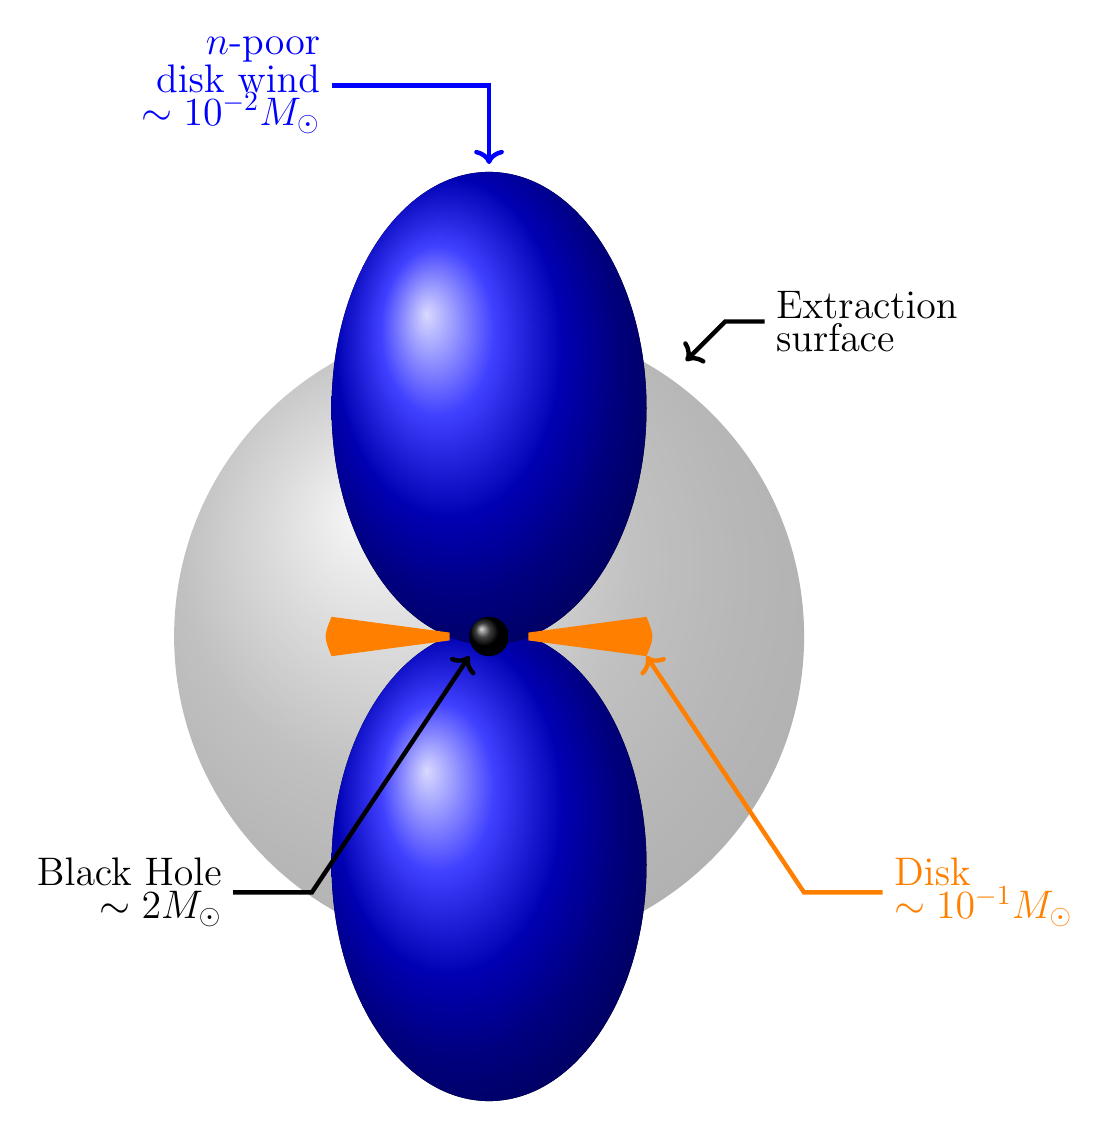
\begin{tikzpicture}
          \tikzfading[name=fade inside,
          inner color=transparent!50,
          outer color=transparent!50]
          
          \coordinate (origin) at (0,0);
          \pgfmathsetmacro{\dbx}{0.5}
          \pgfmathsetmacro{\dby}{0.05}
          \pgfmathsetmacro{\dex}{2.}
          \pgfmathsetmacro{\dey}{0.25}
          \pgfmathsetmacro{\dcc}{2.1}
          \pgfmathsetmacro{\tcx}{5.0}
          
          % extraction surface
          \shade[ball color=gray,path fading=fade inside,opacity=0.75] (origin) circle (4);

          \foreach \i in {-1,1}
          {
            \fill[ball color=blue] (0, \i*2.9) ellipse (2 and 3);
          }
          
          \foreach \i in {-1,1}
          {
            % disk
            \fill[color=orange]
            (\i*\dbx,\dby) -- (\i*\dex,\dey)
            .. controls (\i*\dcc,0) .. (\i*\dex,-\dey)
            -- (\i*\dbx,-\dby) -- cycle;
          }
          
          % bh
          \shade[ball color=black] (origin) circle (0.25);
                    
          % text
          \draw[<-,blue, ultra thick] (0,6) -- ++(0,1) -- ++(-2,0)
          node[left,align=right]
          {\Large \color{blue}$n$-poor\\\Large disk wind\\\Large $\sim 10^{-2}M_{\odot}$};
          
          \draw[<-,orange, ultra thick] (\dex,-\dey)
          -- ++(2,-3) -- ++(1,0)
          node[right,align=left]
          {\Large \color{orange}Disk\\\Large $\sim 10^{-1}M_{\odot}$};
          
          \draw[<-,black, ultra thick] (-0.25,-0.25)
          -- ++(-2,-3) -- ++(-1,0)
          node[left,align=right]
          {\Large \color{black}Black Hole\\ \Large $\sim 2 M_{\odot}$};

          \draw[<-,black,ultra thick] (2.5,3.5)
          -- ++(0.5,0.5) -- ++(0.5,0) node[right,align=left]
          {\Large \color{black}Extraction\\\Large surface};
        \end{tikzpicture}
      }
    \end{column}
  \end{columns}
\end{frame}

\begin{frame}
  \frametitle{Nucleosynthetic Yields}
  \begin{center}
    \includegraphics[height=0.9\textheight]{gw170817-yields-2}
  \end{center}
  {\tiny \textbf{JMM} et al. PRD \textbf{100} 023008 (2019)}
\end{frame}

\begin{frame}
  \frametitle{Spectra}
  \begin{center}
    \includegraphics[height=0.9\textheight]{spectral_evolution}
  \end{center}
  {\tiny \textbf{JMM} et al. PRD \textbf{100} 023008 (2019)}
\end{frame}

\begin{frame}
  \frametitle{Collapsars, and how it all circles back to supernovae}
  \begin{columns}
    \begin{column}{5cm}
      \begin{itemize}
      \item Accretion times $t\sim 10s$
      \item $\dot{M}$ between
        \begin{itemize}
        \item $10^{-4} M_\odot/s$
        \item $10^{-1} M_\odot/s$ 
        \end{itemize}
      \item $\rho \sim 10^{10}$ g$/$cm$^3$
      \end{itemize}
      \resizebox{\columnwidth}{!}{
        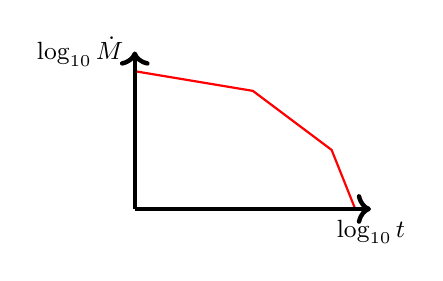
\begin{tikzpicture}
          \draw[thick,red]
          (0,1.75) -- (1.5,1.5) -- (2.5,0.75) -- (2.8,0);

          \coordinate (origin) at (0,0);
          \draw[ultra thick,->]
          (origin) -- ++(3,0)
          node[below] {\small $\log_{10}t$};
          \draw[ultra thick,->]
          (origin) -- ++(0,2)
          node[left] {\small $\log_{10}\dot{M}$};
        \end{tikzpicture}
      }
      \begin{tiny}
        Siegel, Barnes, Metzger. Nature \textbf{241} (2019)
      \end{tiny}
    \end{column}
    \begin{column}{7cm}
      \resizebox{\columnwidth}{!}{
        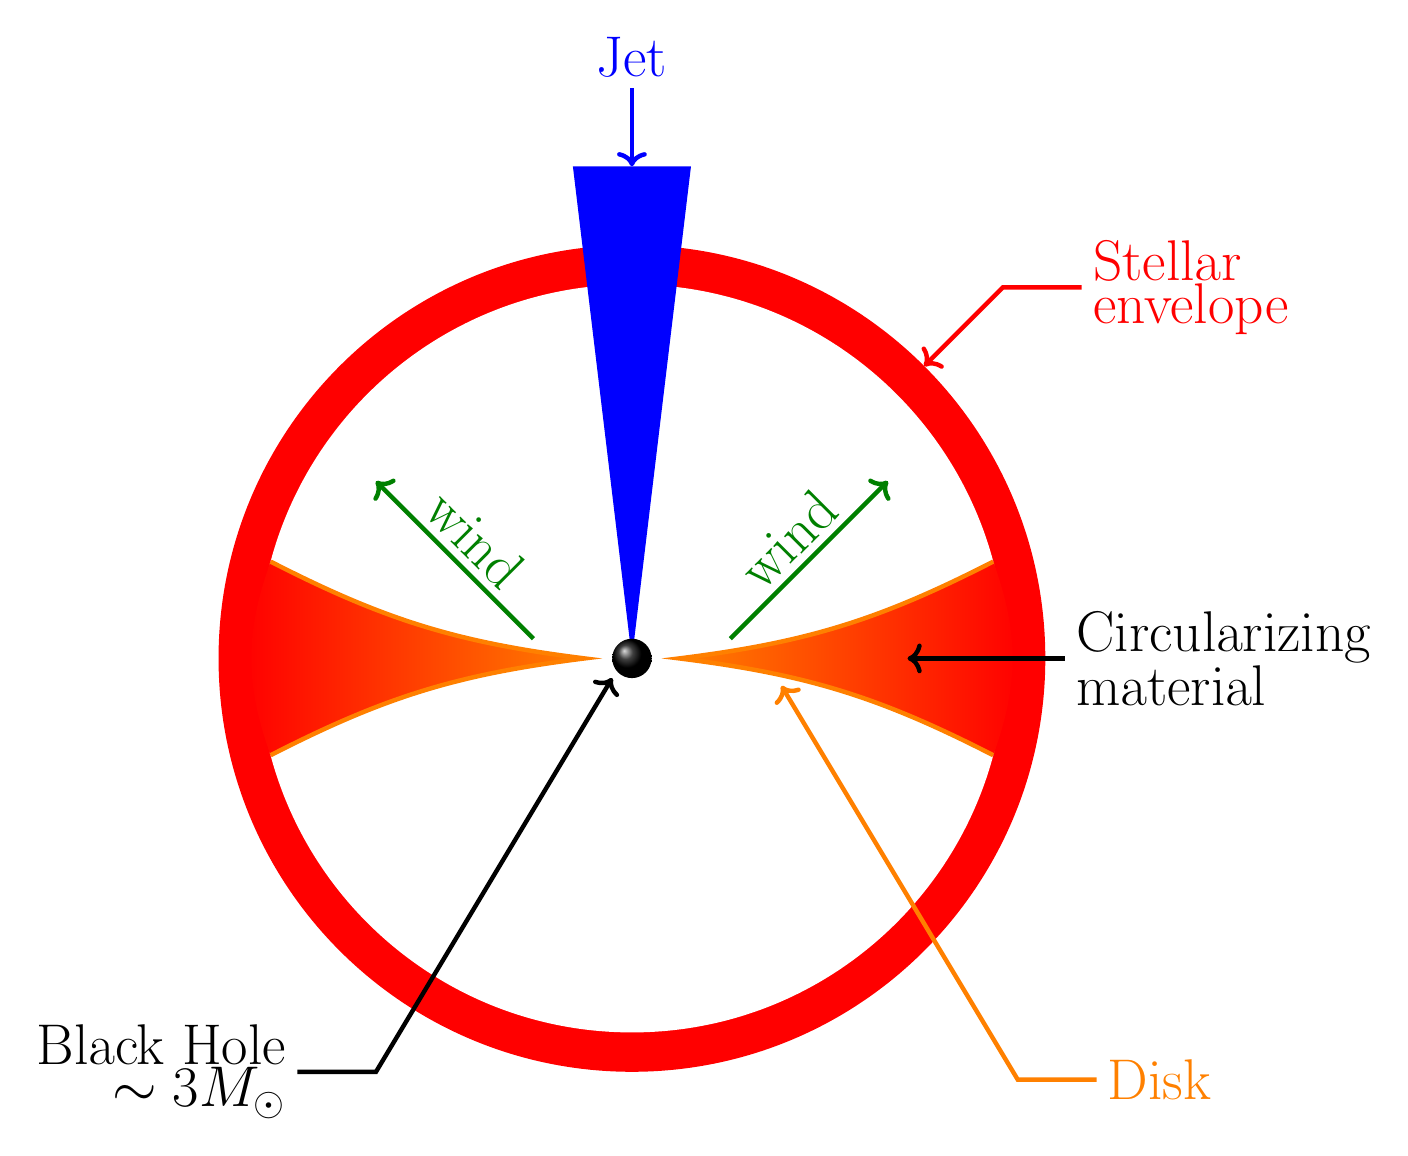
\begin{tikzpicture}
          \coordinate (origin) at (0,0);
          \pgfmathsetmacro{\pi}{3.14159}
          \pgfmathsetmacro{\dbx}{0.5}
          \pgfmathsetmacro{\dby}{0.05}
          \pgfmathsetmacro{\dex}{2.}
          \pgfmathsetmacro{\dey}{0.25}
          \pgfmathsetmacro{\dcc}{2.1}
          \pgfmathsetmacro{\tcx}{5.0}
          \pgfmathsetmacro{\rstar}{5}
          \pgfmathsetmacro{\wstar}{0.25}
          \pgfmathsetmacro{\wjet}{0.75}
          \pgfmathsetmacro{\tangle}{{45}}
          \pgfmathsetmacro{\tsx}{{(\rstar+\wstar)*cos(\tangle)}}
          \pgfmathsetmacro{\tsy}{{(\rstar+\wstar)*sin(\tangle)}}

          \pgfmathsetmacro{\cangle}{15}
          \pgfmathsetmacro{\cx}{(\rstar-\wstar)*cos(\cangle)}
          \pgfmathsetmacro{\cy}{(\rstar-\wstar)*sin(\cangle)}
          % \pgfmathsetmacro{\cend}{\dex + 0.1}
          \pgfmathsetmacro{\cend}{\dbx + 0.1}

          \newcommand{\msize}{\huge}

          % star
          \fill [color=red] (origin) circle (\rstar+\wstar);
          \fill [color=white] (origin) circle (\rstar-\wstar);

          % circularization
          \fill[color=red,
          left color=orange,
          middle color=orange,
          right color=red]
          (\cx,\cy) to [bend left=10] (\cend,0)
          to [bend left=10] (\cx,-\cy)
          to [bend right=20] cycle;
          
          \draw[orange,ultra thick]
          (\cx,\cy) to [bend left=10] (\cend, 0)
          to [bend left=10] (\cx,-\cy);

          \fill[color=red,
          right color=orange,
          middle color=orange,
          left color=red]
          (-\cx,\cy) to [bend right=10] (-\cend,0)
          to [bend right=10] (-\cx,-\cy)
          to [bend left=20] cycle;
          
          \draw[orange,ultra thick]
          (-\cx,\cy) to [bend right=10] (-\cend, 0)
          to [bend right=10] (-\cx,-\cy);

          % \foreach \i in {-1,1}
          % {
          %   % disk
          %   \fill[color=orange]
          %   (\i*\dbx,\dby) -- (\i*\dex,\dey)
          %   .. controls (\i*\dcc,0) .. (\i*\dex,-\dey)
          %   -- (\i*\dbx,-\dby) -- cycle;
          % }
          
          % jet
          \fill[color=blue] (origin) -- (-\wjet,1.25*\rstar) -- ++(2*\wjet,0) -- cycle;

          % bh
          \shade[ball color=black] (origin) circle (0.25);

          % wind
          \draw[deepgreen,ultra thick, ->]
          ({0.5*(\dbx + \dex)},\dey) -- ++(2,2);
          \draw ({0.5*(\dbx + \dex) + 1},{(\dey+1)})
          node[above,align=center,rotate=45]
          {\color{deepgreen}\msize wind};
          \draw[deepgreen,ultra thick, ->]
          ({-0.5*(\dbx + \dex)},\dey) -- ++(-2,2);
          \draw ({-(0.5*(\dbx + \dex) + 1)},{(\dey+1)})
          node[above,align=center,rotate=-45]
          {\color{deepgreen}\msize wind};          

          % text
          \draw[<-,orange, ultra thick] (\dex-0.1,-\dey-0.1)
          -- ++(3,-5) -- ++(1,0)
          node[right,align=left]
          {\msize \color{orange}Disk};
          
          \draw[<-,black, ultra thick] (-0.25,-0.25)
          -- ++(-3,-5) -- ++(-1,0)
          node[left,align=right]
          {\msize \color{black}Black Hole\\ \msize $\sim 3 M_{\odot}$};
          
          \draw[<-,red,ultra thick] (\tsx,\tsy)
          -- ++(1,1) -- ++(1,0)
          node[right,align=left]
          {\msize \color{red} Stellar\\ \msize envelope};

          \draw[<-,blue,ultra thick] (0, 1.25*\rstar) -- ++(0,1)
          node[above,align=center] {\msize \color{blue} Jet};

          \draw[<-,black,ultra thick]
          ({0.5*(\dex+\rstar)},0) -- ++(2,0) node[right,align=left]
          {\msize Circularizing\\ \msize material};
          
          \let\msize\undefined;
        \end{tikzpicture}
      }
    \end{column}
  \end{columns}
\end{frame}

\begin{frame}
  \frametitle{Big Open Questions and Uncertainties}
  \begin{itemize}
  \item Initial conditions matter. What are the right ones? Massive diversity:
    \begin{itemize}
    \item BH mass and spin (V. Urrutia-Hurtado)
    \item Disk mass (S. Curtis)
    \item Magnetic field strength, topology. Transient due to MHD forces real? (K. Lund)
    \item In collapsar case, disk feeding (B. Barker)
    \end{itemize}
  \item Late time physics.
  \item Mapping the central engine to observations (Several topics by itself!)
  \item Neutrino oscillations---Elephant in the room. cm-scale physics impossible to treat.
  \end{itemize}
\end{frame}

\begin{frame}
  \frametitle{Future: Leveraging Next-Generation HPC}
  \begin{columns}
    \begin{column}{6cm}
      \begin{tiny}
      \begin{itemize}
      \item Parthenon AMR library: arXiv:2202.13209
      \item Fast logs: arXiv:2206.08957
      \item spiner performance-portable tables: joss.04367
      \item singularity-eos performance-portable EOS: \url{https://github.com/lanl/singularity-eos}
      \item Phoebus Performance portable GR$\nu$RMHD: \url{https://github.com/lanl/phoebus}
      \end{itemize}
      \end{tiny}
      \begin{center}
        \includegraphics[width=\columnwidth]{parth-hydro-scaling_weak}
      \end{center}
    \end{column}
    \begin{column}{6cm}
      \begin{center}
n        \includegraphics[height=0.9\textheight]{tov_fig_paper}
      \end{center}
    \end{column}
  \end{columns}
\end{frame}

\begin{frame}
  \frametitle{Conclusions}
  \begin{columns}
    \begin{column}{7cm}
      \begin{itemize}
      \item Astrophysical transients are a rich laboratory!
      \item Very big things (stars, supernovae, neutron star mergers)
        tell us a lot about very tiny things (nuclear physics)
      \item Need GRRMHD and neutrino transport!
      \item NS Mergers are awesome!
        \begin{itemize}
        \item Likely source of heavy elements in our
          universe
        \item Disks can produce blue component of kilonova
        \end{itemize}
      \item Stay tuned for more
      \end{itemize}
    \end{column}
    \begin{column}{5cm}
      \includegraphics[width=\columnwidth,clip,trim={150 0 150 0}]{3d_render}
    \end{column}
  \end{columns}
\end{frame}

\backupbegin

\begin{frame}
  \frametitle{The story differs for more massive disks, BHNS Mergers}
  \begin{columns}
    \begin{column}{8cm}
      Remnant + Disk parameters, chosen to sample edge of what's possible:
      \begin{itemize}
      \item $M_{BH}=10, a = 0.8, M_d=0.082$\vspace{0.95cm}
      \item $M_{BH}=6, a = 0.75, M_d=0.1425$\vspace{1cm}
      \item $M_{BH}=7, a = 0.9, M_d=0.25$\vspace{0.95cm}
      \item $M_{BH}=5, a = 0.9, M_d=0.42$\vspace{0.85cm}
      \end{itemize}
      {\footnotesize Curtis, \textbf{JMM}, Frohlich. In Prep.}
    \end{column}
    \begin{column}{4cm}
      \begin{center}
        \includegraphics[height=0.9\textheight,clip,trim={0 0 0 0.25cm}]{nsbh_disks_rho_ye}
      \end{center}
    \end{column}
  \end{columns}
\end{frame}

\begin{frame}
  \frametitle{Electron Fractions and Yields}
  \begin{columns}
    \begin{column}{6cm}
      \begin{center}
        \includegraphics[width=\columnwidth]{bhns_curtis/ye_hist}
      \end{center}
    \end{column}
    \begin{column}{6cm}
      \begin{center}
        \includegraphics[width=\columnwidth]{bhns_curtis/total_abun_disks_aug22}\\
      \end{center}
    \end{column}    
  \end{columns}
  {\footnotesize Curtis, \textbf{JMM}, Frohlich. In Prep.}
\end{frame}

\begin{frame}
  \frametitle{Preliminary: Black hole spin influences jet + wind}
  \begin{itemize}
  \item Black hole properties, such as spin change jet opening angle, and interaction of jet with wind.\\(Preliminary. V. Urrutia-Hurtado et al.)
  \end{itemize}
  \begin{columns}
    \begin{column}{6cm}
      \begin{center}
        \includegraphics[width=\columnwidth]{jet-opening/sigmaconxz5799_lvl1_800}
      \end{center}
    \end{column}
    \begin{column}{6cm}
      \begin{center}
        \includegraphics[width=\columnwidth]{jet-opening/thwsigbigger}
      \end{center}
    \end{column}
  \end{columns}
\end{frame}

\begin{frame}
  \frametitle{Collapsar Disks: A Cautionary Tail}
  \resizebox{12cm}{!}{
    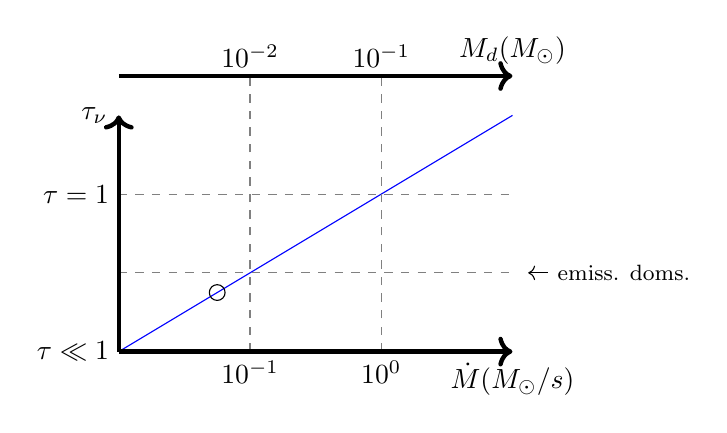
\begin{tikzpicture}
      \coordinate (origin) at (0,0);

      \draw[blue] (origin) -- (5,3);

      \node[left] (tau1) at (0,2) {$\tau=1$};
      \draw[dashed,gray] (tau1) -- ++(5.5,0);

      \node[below] (m1) at (10./3.,0) {$10^0$};
      \draw[dashed,gray] (m1) -- ++(0,3.75)
      node[above] {\color{black}$10^{-1}$};
      
      \coordinate(tau2) at (0,1);
      \draw[dashed,gray] (tau2) -- ++(5,0);

      \node[below](m2) at (5./3.,0) {$10^{-1}$};
      \draw[dashed, gray] (m2) -- ++(0, 3.75)
      node[above] {\color{black}$10^{-2}$};

      \node[left] at (origin) {$\tau\ll 1$};
      \draw[ultra thick, black,->] (origin)
      -- ++(5, 0) node[below] {$\dot{M} (M_\odot/s)$};
      \draw[ultra thick, black, ->] (origin)
      -- ++(0, 3) node[left] {$\tau_\nu$};
      \draw[ultra thick, black, ->] (0,3.5)
      -- ++(5,0) node[above] {$M_d (M_\odot)$};

      \draw[<-] (5.2,1) -- ++(0.25,0) node[right,align=left]
      {\footnotesize emiss. doms.};

      \draw (5./4.,3./4.) circle (0.1);
    \end{tikzpicture}
    }
\end{frame}

\begin{frame}
  \frametitle{Electron Fraction With and Without Absorption}
  \begin{columns}
    \begin{column}{6cm}
      \begin{itemize}
      \item Electron Fraction With Absorption
      \end{itemize}
      \begin{center}
        \includegraphics[height=7cm]{collapsar/ye_v_theta}
      \end{center}
    \end{column}
    \begin{column}{6cm}
      \begin{itemize}
      \item Electron Fraction With Optically thin Cooling
      \end{itemize}
      \begin{center}
        \includegraphics[height=7cm]{collapsar/ye_em_v_theta}
      \end{center}
    \end{column}
  \end{columns}
\end{frame}

\begin{frame}
  \frametitle{Absorption and Initial Conditions}
  \begin{center}
    \resizebox{12cm}{!}{
      \begin{tikzpicture}
        \node[inner sep=0pt] (id) at (-3, 2)
        {\includegraphics[width=6cm]{collapsar/close/anim_RHO/frame_0001}};
        \node[inner sep=0pt] (ts) at (3, -1)
        {\includegraphics[width=6cm]{collapsar/ye_statistics}};
        \node[inner sep=0pt] (opac) at (-3, -2)
        {\includegraphics[width=6cm]{collapsar/transient-dtau}};
        \draw[ultra thick,red,->] (-1,2) -- (1.5, 0.5);
        \draw[ultra thick, red,->] (-3,1) -- (-3, -1);
      \end{tikzpicture}
    }
  \end{center}
  {\footnotesize Miller et al., ApJ \textbf{902}, 66 (2020)}
\end{frame}

\begin{frame}
  \frametitle{How is $Y_e$ vs Lattitude Set?}
  \begin{itemize}
  \item Traced paths of Lagrangian fluid packets through the disk.
  \end{itemize}
  \begin{center}
    \includegraphics[width=0.9\textwidth]{collapsar/selected_traces_lattitude_cut}
  \end{center}
  {\footnotesize Miller et al., ApJ \textbf{902}, 66 (2020)}
\end{frame}

\begin{frame}
  \frametitle{Turbulence and $Y_e$}
  \resizebox{12cm}{!}{
    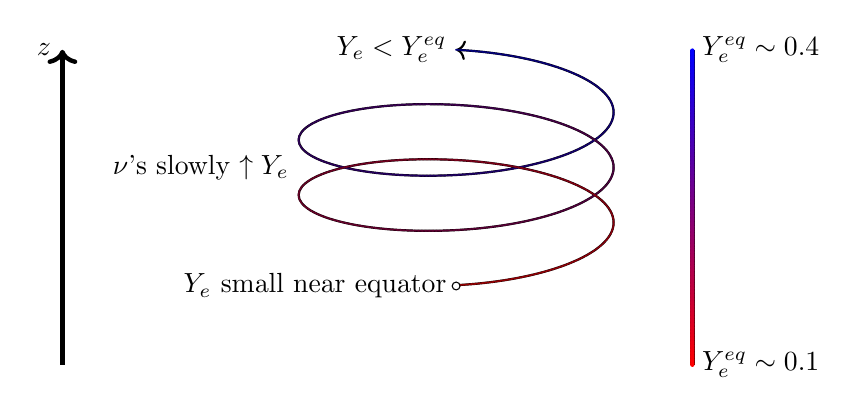
\begin{tikzpicture}
      \coordinate(origin) at (-2,0);

      \draw[ultra thick, black, ->] (origin) -- ++ (0, 4)
      node[left] {$z$};

      \draw[ultra thick,colormorph={0.8pt}{red}{blue}] (6,0) -- ++(0,4);
      \node[right] at (6,0) {$Y_e^{eq}\sim 0.1$};
      \node[right] at (6,4) {$Y_e^{eq}\sim 0.4$};

      \draw[thick,
      decoration={aspect=0.31,segment length=7mm,amplitude=2cm, coil},
      colormorph={0.4pt}{deepblue}{deepred},
      decorate,arrows={<[bend]-}] (3,4) -- (3,1);
      \node[draw,fill=white,circle,inner sep=1pt] at (3,1) {};
      \node[left] at (3,1) {$Y_e$ small near equator};
      \node[left] at (1.,2.5) {$\nu$'s slowly $\uparrow Y_e$};
      \node[left] at (3,4) {$Y_e < Y_e^{eq}$};
    \end{tikzpicture}
  }
\end{frame}

\begin{frame}
  \frametitle{$Y_e$ is set by the balance of Turbulence and
    Neutrinos!}
  \begin{center}
    \includegraphics[width=0.9\textwidth]{collapsar/ye_time_scales_t5000}
  \end{center}
  {\footnotesize Miller et al., ApJ \textbf{902}, 66 (2020)}
\end{frame}

\begin{frame}
  \frametitle{$Y_e$ is set by the balance of Turbulence and
    Neutrinos!}
  \begin{center}
    \includegraphics[height=0.9\textheight]{collapsar/model-vs-vertical-structure}    
  \end{center}
  {\footnotesize Miller et al., ApJ \textbf{902}, 66 (2020)}
  \end{frame}

\begin{frame}
  \frametitle{$Y_e$ is set by the balance of Turbulence and
    Neutrinos!}
  \begin{displaymath}
      Y_{\rm e}(z/H) = \braket{\text{min}(Y_{\rm e})}_{\text{trc}}
      + \braket{\frac{d Y_{\rm e}}{dt}}_{t,\text{trc}} \paren{H\braket{\frac{dz}{dt}}_{t,\text{trc}}^{-1}}\paren{\frac{z}{H} - \braket{\text{min}(z/H)}_{\text{trc}}}
    \end{displaymath}
    \begin{columns}
      \begin{column}{6cm}
        \includegraphics[width=\columnwidth]{collapsar/vertical-structure-params}
      \end{column}
      \begin{column}{6cm}
        \includegraphics[width=\columnwidth]{collapsar/model-vs-vertical-structure}
      \end{column}
    \end{columns}
    {\footnotesize Miller et al., ApJ \textbf{902}, 66 (2020)}
  \end{frame}

\begin{frame}
  \frametitle{Future}
  \begin{itemize}
  \item Large optical depths, such as inside a neutron star present issues for Monte Carlo
  \item Need a method that can span the range of optical depths and solve the full transport equation
  \item Great progress community. See work by Radice, Mullen, Foucart, others.
  \end{itemize}
  \begin{center}
    \includegraphics[width=\textwidth]{mocmc-diagram};
  \end{center}
  {\footnotesize Ryan and Dolence, ApJ \textbf{891} 118 (2020)}
\end{frame}

\backupend

\end{document}